\documentclass[ngerman,runningheads]{llncs}

%---- Sonderzeichen-------%
\usepackage {ngerman}
%---- Codierung----%
\usepackage[utf8x]{inputenc}	% for Unix and Windows
\usepackage[T1]{fontenc}
\usepackage{graphicx}
\usepackage{url}
\usepackage{llncsdoc}
%----- Mathematischer Zeichenvorrat---%
\usepackage{amsmath}
\usepackage{amssymb}
\usepackage{enumerate}
% fuer die aktuelle Zeit
\usepackage{scrtime}
\usepackage{listings}
\usepackage{subfigure}
\usepackage{hyperref}

\setcounter{tocdepth}{3}
\setcounter{secnumdepth}{3}


\begin{document}

\mainmatter
\title{Änderungsgetriebene Konsistenz zwischen Java-Code und Software-Architekturmodellen}
\titlerunning{Praktikum Software Quality Engineering mit Eclipse} \author{Thomas Czogalik}
\authorrunning{Thomas Czogalik}
\institute{Betreuer: Heiko Klare, Max Kramer}
\date{12.10.2017}
\maketitle


\section{Einleitung}
Das Praktikum \texttt{Software Quality Engineering mit Eclipse} fand im Sommersemester 2017 statt. Mein Thema war \texttt{Änderungsgetriebene Konsistenz zwischen Java-Code und Software-Architekturmodellen} und wurde von Heiko Klare und Max Kramer vom Lehrstuhl Software Design and Quality (SDQ) betreut. \par
Bei der Entwicklung eines Software-Systems können verschiedene Modelle, auf unterschiedlichen Abstraktionsebenen zum Einsatz kommen, um dieses zu beschreiben. Die dargestellten Informationen können voneinander abhängig und redundant sein. Entwickler müssen bei Änderungen an einem Modell evtl. auch Änderungen an anderen Modelle vornehmen, damit diese konsistent bleiben. Automatisierte Verfahren sind für diese Konsistenzwiederherstellung nötig, da ein Entwickler kaum in der Lage ist den Überblick über alle Abhängigkeiten zu behalten. Einen solchen Ansatz verfolgt Vitruvius \cite{kramer2013b}. Durch einen änderungsgetriebenen Ansatz und verschiedener Transformationssprachen, können verschiedene Modelle automatisch konsistent gehalten werden.
%Ziel des Praktikums war es die Konsistenzerhaltung zwischen Java-Code und PCM-Elementen mithilfe der Reaction-Sprache umzusetzen und damit die bestehende Java Implementierung zu ersetzen. Die bereits existierenden JUnit Tests stellten dabei sicher, dass das Verhalten gleich bleibt. \par
%Vitruvius steht für VIew-cenTRic engineering Using a VIrtual Underlying Single model. Der Ansatz basiert auf einem Orthographischen Software Modell (OSM) basierend auf dem Konzept von Atkinson et. al. \cite{Atkinson2010}. Es besteht nicht aus einem einzelnen zugrundeliegend Meta Modell (SUM), sondern bestehende Meta-Modelle werden zu einem modularem zugrundeliegenden Modell kombiniert. \par
Eine solche Transformationssprache ist die Reactions-Sprache \cite{kramer2017a}. Die Reactions-Sprache ist eine Domänenspezifischesprache (DSL) um Konsistenzbeziehungen zwischen Metamodellen zu beschreiben. Sie besteht aus Reactions und Routinen. Reactions definieren wann Konsistenzerhaltungslogik ausgeführt werden soll. Routinen definieren dabei wie die Konsistenz (wieder) hergestellt wird. Dabei können Routinen von Reactions oder anderen Routinen aufgerufen werden und können wiederverwendet werden. \autoref{img:reaction} zeigt ein Beispiel für eine solche Reaction. Dabei wird in der Reaction zunächst definiert, wann diese ausgeführt werden soll. Die Reaction wird ausgeführt, wenn ein Java-Interface in ein Java-Paket eingefügt wird. Wenn dies der Fall ist, soll eine Routine mit dem Namen \texttt{createPCMInterface} aufgerufen werden. Diese Routine erstellt ein PCM-Interface und initialisiert es mit dem gleichen Namen wie das Java-Interface. Im Anschluss wird noch eine Korrespondenz zwischen beiden Elementen erstellt, damit man zwischen ihnen navigieren kann. Dies ist unter anderem nötig, wenn zum Beispiel Änderungen an einem der beiden Elemente durchgeführt werden.
\begin{figure}[htp]
	\centering
  	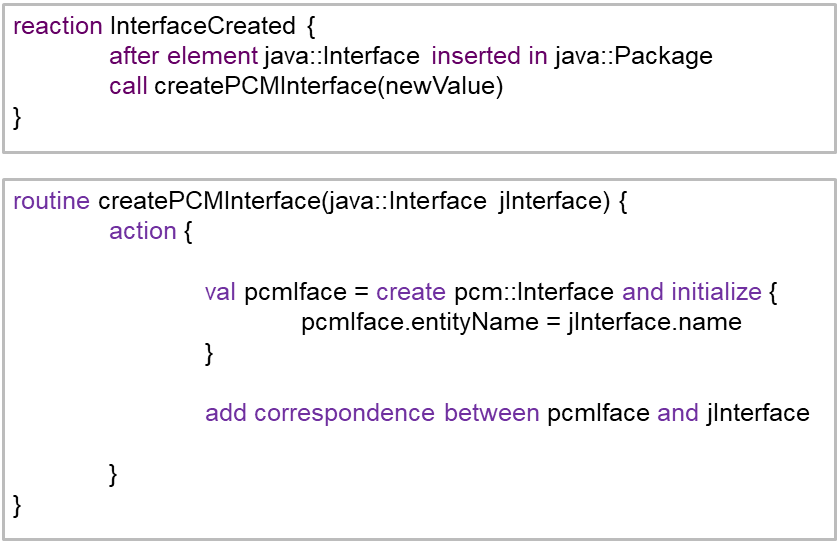
\includegraphics[width=1\textwidth]{images/reaction.png}
	\caption{Beispiel für eine Interface-Reaction in der Reactions-Sprache}
	\label{img:reaction}
\end{figure} \par
Im Folgenden wird ein Überblick über das Praktikum gegeben. Dabei wird in \autoref{sec:tätigkeit} beschrieben was meine Aufgaben waren und das Ergebnis präsentiert. In \autoref{sec:probleme} werden Probleme mit dem Ergebnis beschrieben. \autoref{sec:auswertung} bewertet die Reactions-Sprache und das Praktikum. Schließlich wird in \autoref{sec:ausblick} beschrieben, wie es mit der Implementierung nach dem Praktikum weitergehen und wie die Reactions-Sprache erweitert werden kann. 
\section{Tätikgeit}
\label{sec:tätigkeit}
Im Folgenden Abschnitt werden die Aufgaben und das Ergebnis des Praktikums beschrieben. \par
Die Hauptaufgabe des Praktikums war es die Konsistenzerhaltung zwischen Java-Code und PCM-Elementen mithilfe der Reactions-Sprache umzusetzen und damit die bestehende Java Implementierung zu ersetzen. Gleichzeitig sollte evaluiert werden wie gut das mit der Reactions-Sprache möglich ist und wo es noch Probleme oder Verbersserungsmöglichkeiten gibt. Die Java Implementierung war, zu großen Teilen, durch JUnit-Plugin-Tests getestet worden. Diese Tests sollten sicherstellen, dass das Verhalten gleich bleibt, wenn die Implementierung ausgetauscht wird. Ein JUnit-Plugin-Test bietet die Möglichkeit ein Plugin in einer eigenen virtuellen Maschine zu starten. In dieser Instanz wird der Test gestartet. Damit verschiedene Modelle konsistent gehalten werden können, benötigt es zunächst Regeln, die die Elemente des einen Modells auf Elemente des anderen Modells abbilden. Die Abbildungsregeln für Java-Code und PCM-Elemente sind in \autoref{img:mapping} abgebildet. Diese stammen aus der Dissertation von Michael Langhammer \cite{langhammer}. Dort kann auch eine genauere Beschreibung der Zuordnung gefunden werden.
\begin{figure}[htp]
	\centering
  	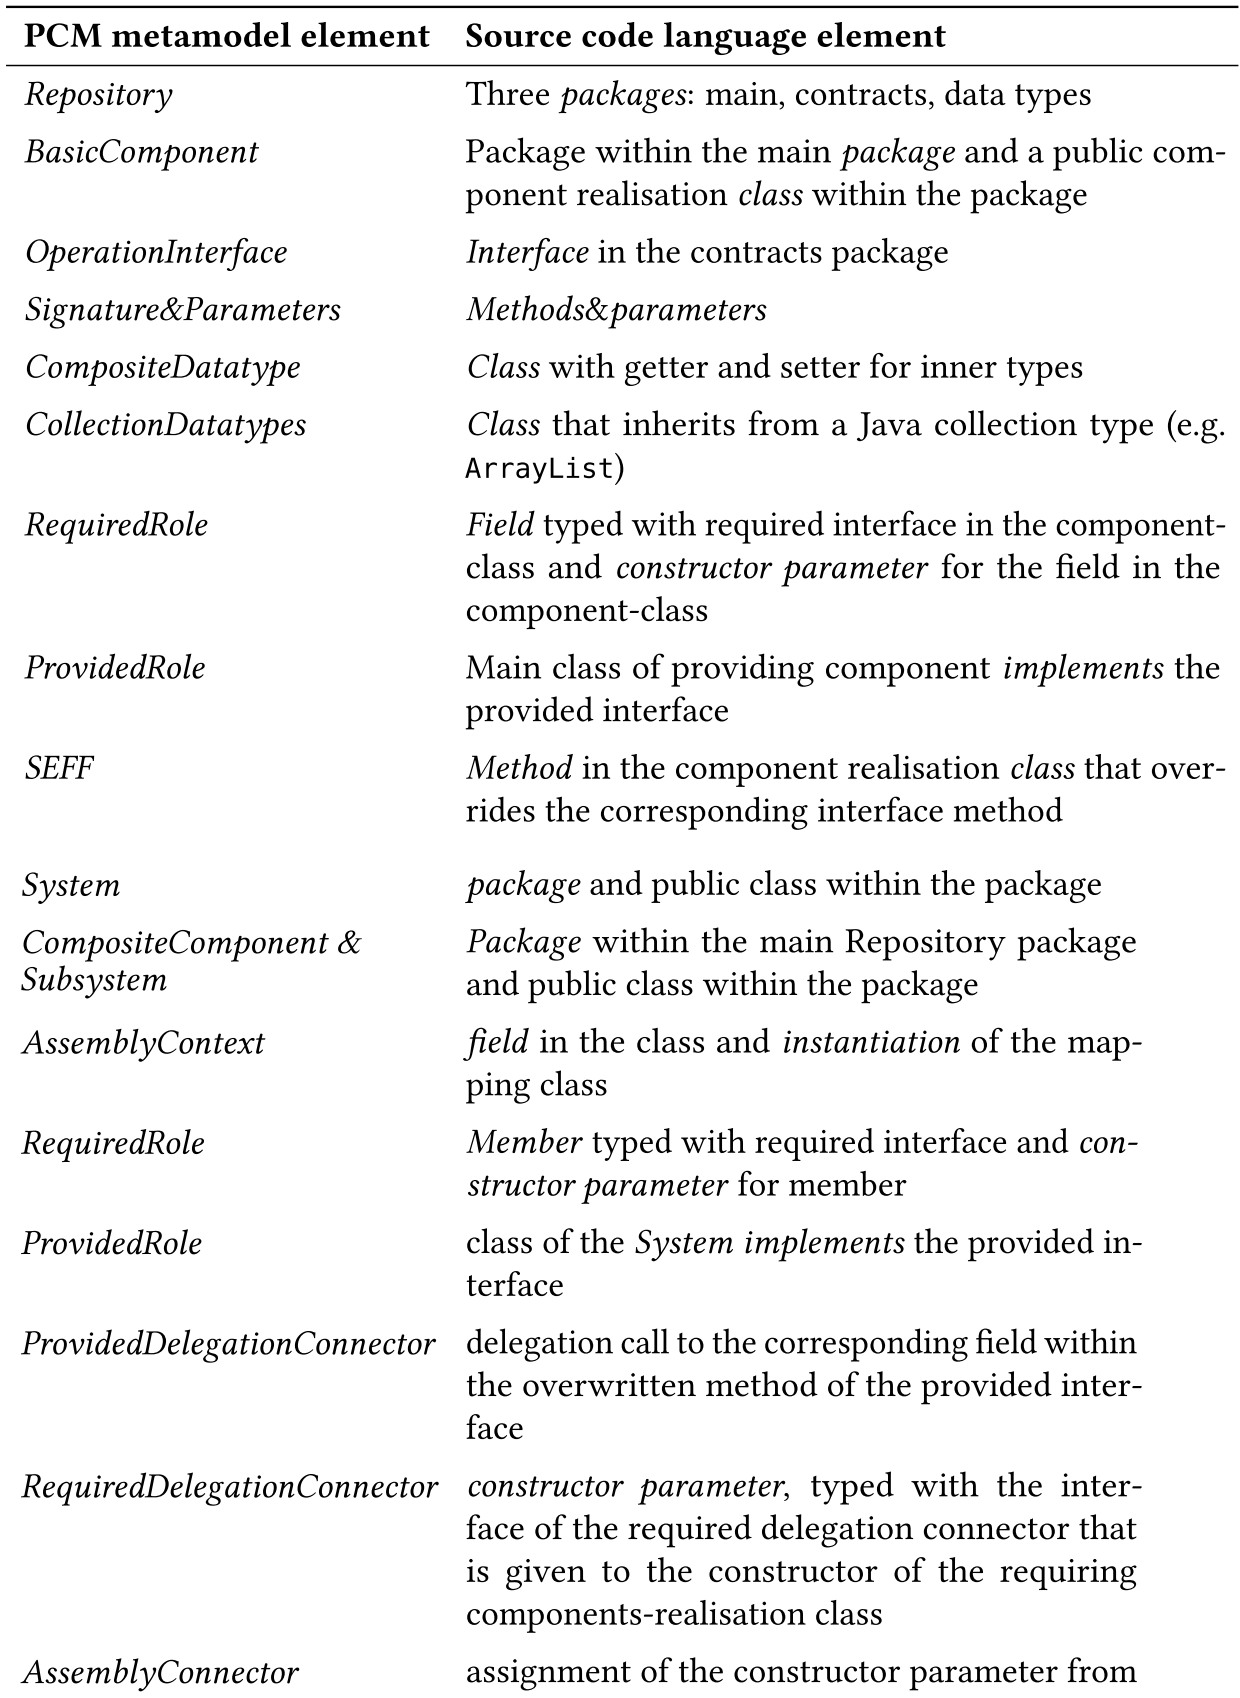
\includegraphics[width=1\textwidth]{images/mapping.png}
	\caption{Übersicht der Zuordnung von PCM-Elementen und Java-Code}
	\label{img:mapping}
\end{figure} 
%\begin{table}
%\centering
%\begin{tabular}{l|l}
%\multicolumn{2}{l}{\textit{}}
%\\\hline
%\textbf{PCM Meta-Modell Element} & \textbf{Java-Modell Element} \\\hline
%%Repository & Drei Pakete: main, contracts, datatypes \\
%\hline
%BasicComponent & Paket im main-Paket und eine öffentliche Klasse in dem Paket \\
%\hline
%OperationInterface & Schnittstelle im contracts-Paket \\
%\hline
%%%Signature\&Parameters & Methoden und Parameter \\
%\%hline
%CompositeDatatype & Klasse mit getter und setter für innere Typen \\
%\hline
%CollectionDatatype & Klasse erbt von Java-Collection Typ (z.B. Arraylist) \\
%\hline
%RequiredRole & Feld mit Typ einer requiered-Schnittstelle in einer Komponentenklasse und \\
% & Konstruktorparameter \\
%\hline
%ProvidedRole & Klasse implementiert angebotene Schnittstelle \\
%\hline
%SEFF & Methode die eine Methode einer Schnittstelle überschreibt \\
%\hline
%&System & Paket im main-Paket und eine öffentliche Klasse in dem Paket \\
%\hline
%\end{tabular}
%\caption{\label{tab:gqm}Ziele, Fragen und Metriken für die Validierung, nach der GQM-%Methode}
%\end{table}
Außerdem wurden die beiden Arbeiten von Max Kramer \cite{kramer2017a} und Heiko Klare \cite{klare2016} benutzt um ein Verständnis für die Reactions-Sprache zu erhalten. Im Anschluss wurde die Java Implementierung analysiert und nach und nach durch Reactions und Routinen ausgetauscht. Mithilfe der bestehenden Tests wurde die Reactions-Implementierung fortlaufend validiert. Jede Testklasse validierte dabei eine Abbildungsklasse. D.h. die Testklasse \texttt{ClassMappingTest} validiert alle Abbildungsregeln die mit Java-Klassen zu tun haben. Die Tests sind so aufgebaut, das jede mögliche Zuordnung aus \autoref{img:mapping} einmal getestet wird. Außerdem gibt es Tests für einige Editierfunktionen, wie das Umbenennen von Elementen. \par
%Tests für das Löschen von Elementen waren nicht umgesetzt. Sie wurden auch im Rahmen des Praktikums nicht umgesetzt, da dies nicht Teil des Praktikums war. \par
Im Ergebnis wurden die Abbildungsregeln für Repositories, Komponenten, Systeme, Datatypes, Rollen und den SEFF (Service Effect Specification) umgesetzt. Zudem wurde gegen Ende des Praktikums bemerkt, dass nicht alle Abbildungsregeln der Java Implementierung getestet wurden. Dazu gehören der SEFF Inhalt, AssemblyContext und AssemblyConnector. Außerdem wurden einige Editierfunktionen, wie das Löschen oder Ändern von Elementen nicht vollständig getestet. Da das Erstellen von Tests nicht Teil des Praktikums war, wurde entschieden sich zunächst auf die vorhandenen Tests und die damit einhergehenden Reactions zu konzentrieren. \par 
Die Implementierung besteht dabei aus zwei Reactions-Dateien, die für unterschiedliche Arten von Reaktionen verantwortlich sind. In \texttt{Java2PcmClassifier} befinden sich alle Reactions, die ausgelöst werden, wenn Pakete, Klassen, Schnittstellen oder Typreferenzen erstellt werden. In \texttt{Java2PcmMethods} befinden sich alle Reactions, die ausgelöst werden, wenn Parameter, Felder, Methoden erstellt oder Elemente umbenannt werden. Eine Hilfsklasse bietet zudem Helfermethoden an, die benötigt werden um zum Beispiel Referenzen aufzulösen oder bestimmte Elemente zu filtern. Diese Methoden sind nötig, da ihre Funktionalität nicht mit der Reactions-Sprache umsetzbar ist. In \autoref{sec:reaction} wird näher auf die Hilfsklasse eingegangen. Außerdem befinden sich in \\ \texttt{Java2PcmUserSelection} alle möglichen Auswahlmöglichkeiten die der Benutzer im Lauf der Konsistenzerhaltung haben kann, um zwischen bestimmten Reaktionen auswählen zu können. Auf Github \footnote{https://github.com/vitruv-tools/Vitruv-Applications-ComponentBasedSystems} kann die Implementierung eingesehen werden. Außerdem mussten die Tests teilweise angepasst werden. Dies war nötig da sie zum einen sehr an die Java Implementierung gekoppelt waren und zum Anderen bereits mit der Java Implementierung nicht funktioniert haben. Außerdem ermöglichten die Tests bestimmte Benutzerinteraktion nicht und mussten deshalb erweitert werden. Im Ergebniss laufen fast alle Tests erfolgreich durch. Auf die fehlerhaften Tests wird in \autoref{sec:probleme} eingegangen. \par
Um das Ergebnis, neben den Tests, weiter zu validieren und um weiteres Feedback zu erhalten wurde gegen Ende des Praktikums ein Code-Review vorbereitet und durchgeführt. Im Anschluss wurden die Ergebnisse des Reviews in die Implementierung eingebaut. \par
\section{Probleme}
\label{sec:probleme}
In diesem Abschnitt soll auf noch bestehende Probleme mit dem Ergebnis eingegangen werden. \par
Eines der Ziele des Praktikums war es, dass neben der Umsetzung der Reaktionen mit der Reactions-Sprache auch alle vorhandenen Tests weiterhin erfolgreich durchlaufen und sich das Verhalten des Systems nicht ändert. Dieses Ziel ist schwierig zu validieren, da einige Tests aus nicht bekannten Gründen manchmal fehlschlagen und beim zweiten Ausführen erfolgreich durchlaufen. Mögliche Ursachen für das Scheitern sind zum Beispiel zu lange Wartezeiten auf asynchrone Tasks. Außerdem kann die TUID nicht immer aufgelöst oder das korrespondierende Element nicht gefunden werden. Eine TUID (temporary unique identifier) ist ein eindeutiger Identifizierer für Modellelemente über mehrere verschiedene Modelle hinweg. Führt man diese fehlgeschlagenen Tests nochmal oder einzeln aus, taucht der Fehler nicht mehr auf. Dieses Verhalten war bereits vor dem Praktikum und in anderen Bereichen des Projekts zu beobachten. \par
Ein weiteres Problem, im Ergebnis, ist das nicht immer die Reaction ausgelöst wird, die erwartet wird. Dies ist vor allem ein Problem beim Ändern von Parametern. Wird ein Parameter in einer Signatur verändert, wird zunächst ein neuer Parameter angelegt und im Anschluss der Alte gelöscht. Somit wird nicht ein Änderungs-Event sondern ein Hinzufüge- und Entfern-Event ausgelöst. Noch dazu wird beim Entfernen ein fehlerhafter Parameter vom Monitor geliefert. Dies konnte bis zum Abschluss des Praktikums nicht behoben werden.
\section{Auswertung}
\label{sec:auswertung}
Im Folgenden wird zunächst die Reactions-Sprache und im Anschluss das Praktikum ausgewertet.\par
\subsection{Reactions-Sprache}
\label{sec:reaction}
Ich finde, dass die Reactions-Sprache durch ihren Aufbau und die verschiedenen Konstrukte einfach zu verstehen ist, da sie sich fast wie natürliche Sprache lesen lässt. Dadurch können nach ein paar Beispielen bereits die ersten Reactions geschrieben werden. Die verschiedenen Konstrukte führen dazu, dass der Reaction-Code kompakter wird und sich der Benutzer der Sprache um viele Dinge nicht kümmern muss. Ein Beispiel ist hier das Konstrukt \texttt{retrieve correspondence} um das korrespondierende Element zu erhalten. Während dies in der Reactions-Sprache innerhalb einer Zeile geht, müssen in Java mehrere Hilfsmethoden aus unterschiedlichen Bibliotheken und Null-Checks aufgerufen werden. Solche Konstrukte führen dazu, dass der Reactions-Code aus ca. 960 Zeilen, während der ursprüngliche Java-Code aus ca. 1420 Zeilen besteht. Trotzdem weisen die Reactions die gleiche Funktionalität auf wie die ursprüngliche Java-Implementierung, da alle Tests erfolgreich sind, unter Beachtung von \autoref{sec:probleme}. Somit kann die Reactions-Implementierung die Java-Implementierung ersetzen. \par
%Mit \texttt{retrieve correspondance} kann zum Beispiel innerhalb einer Zeile das korrespondierende Element erhalten werden, während in Java mehrere Hilfsmethoden und Null-Checks aufgerufen werden müssen. Dieses Konstrukt findet sich in einem \texttt{match}-Block wieder, der am Anfang einer Routine steht. Findet sich nämlich z.B. keine Korrespondenz, wird der restliche Teil der Routine nicht ausgeführt. Dadurch lassen sich einige If-Else-Konstrukte ersetzen, indem die jeweiligen Routinen hintereinander aufgerufen werden und nur die passende, bei der der match-Block greift ausgeführt wird. Allein mit diesem Mechanismus konnten einfache Abbildungsregeln, wie Java-Interface auf PCM-Interface, mit wenig Code umgesetzt werden. Wenn eine Abbildungsregel doch komplizierter ist, wie zum Beispiel die der Java-Klasse, kann innerhalb von Routinen auch Xtend Code ausgeführt werden und auch andere Hilfsmethoden aufgerufen werden. \par
Trotz der genannten Vorteile musste neben den Reactions eine Hilfsklasse genutzt werden. Von den 960 Zeilen ist die Hilfsklasse für 180 Zeilen verantwortlich. Die Hilfsklasse ist nötig, da bestimmte Funktionalitäten von der Reactions-Sprache nicht unterstützt werden. Eine solche Funktionalität ist, dass Routinen keine Rückgabewerte haben. In meiner Implementierung musste ich deshalb eine Hilfsmethode für das Extrahieren eines Paketnamens und für das vergleichen von Signaturen schreiben. Hier muss jedoch diskutiert werden, ob dies überhaupt gewollt ist, dass Routinen Rückgabewerte haben sollen. Neben diesen Methoden ist ein Großteil der Hilfsklasse dafür da um Typreferenzen aufzulösen. Vor allem hier könnte der Code deutlich reduziert werden, weil das Auflösen von Referenzen in allen Modellen auftaucht. Ein Sprachkonstrukt oder sogar eine automatische Auflösung im Hintergrund wäre hier hilfreich, da sonst der Benutzer sich um jede Auflösung selber kümmern muss. Neben der Hilfsklasse verursacht die Benutzerinteraktion viel ähnlichen Code. Eine Benutzerinteraktion besteht aus drei Teilen. Zuerst wird die Nachricht und die Möglichkeiten erstellt. Dann wird die Benutzerinteraktion initiiert. Schließlich werden je nach Eingabe unterschiedliche Aktionen ausgeführt. Diese Schritte werden momentan in Xtend-Code geschrieben. Ein Konstrukt, dass dem Nutzer der Sprache hilft diese drei Schritten zu definieren, wäre hier hilfreich und weniger fehleranfällig, bei der Definition, als Xtend-Code. Außerdem ist es nicht möglich Routinen zu überladen. Dies führt dazu das anstatt zum Beispiel einer Routine \texttt{createElement} mit Parameter \texttt{pcm::Repository} oder \texttt{pcm::BasicComponent} jedes Mal ein neuer Name gewählt werden muss. Dies führt nicht unbedingt zur Lesbarkeit bei, da man direkt in der Signatur erkennen kann, was der Zweck dieser Routine ist. \par
%Eine weitere Verbesserung sehe ich in der Routinen Signatur. In \autoref{img:typeguard:before} wird mithilfe von \texttt{with} geprüft ob das übergebene Element nur vom Typ eines der beiden Untertypen von \texttt{Typereference} ist. 
%\begin{figure}[htp]
%%	\centering
%  	\includegraphics[width=1\textwidth]{images/typeguards_before.png}
%	\caption{Mithilfe von \texttt{with} muss der Typ überprüft werden.}
%	\label{img:typeguard:before}
%\end{figure}
%\begin{figure}[htp]
%	\centering
 % 	\includegraphics[width=1\textwidth]{images/typeguards_after.png}
%	\caption{Mit Typeguards kann die gleiche Routine für mehrere definierte Typen verwendet werden.}
%	\label{img:typeguard:after}
%\end{figure}
%Dies könnte mithilfe von Typeguards wie sie zum Beispiel in Typesript verwendet werden umgesetzt werden. Eine mögliche Umsetzung ist in \autoref{img:typeguard:after} abgebildet. Dabei werden in der Routinen Signatur Mögliche Typen definiert. Dies ist auch hilfreich, wenn die Typen keinen gemeinsamen Obertyp haben, und die Implementierung der Routine unabhängig von den Typen ist. 
Neben den Sprachfunktionalitäten muss der Editor für die Reactions-Sprache angepasst und erweitert werden. Dieser unterstützt nämlich wenig Funktionen aus dem Eclipse-Kontext. Zu den fehlenden Funktionen zählen ein Formatierer, eine Autovervollständigung und die Refaktorierung von Name, aber auch zum Beispiel das extrahieren von Routinen. Diese Funktionalitäten sind mir besonders aufgefallen, da ich diese, bei der Nutzung von Eclipse, häufig verwende. Weiter Nutzerstudien oder Praktika könnten ähnliche oder andere Funktionen offenbaren, die Benutzer der Reactions-Sprache benötigen. Durch das Bereitstellen dieser Editor Funktionen könnte die Benutzung der Reactions-Sprache noch einfacher werden, da diese im Eclipse Kontext erwartet werden.\par
%Ich finde, dass die Sprache Grundsätzlich einfach zu lernen und zu verstehen ist, da sie vorallem bei einfachen Reactions wie natürliche Sprache gelesen werden kann. Außerdem konnte durch die Reaction-Sprache die Java-Implementierung ersetzt und die Funktionalität verständlicher gemacht werden. Auch der Code konnte deutlich reduziert werden. Trotzdem gibt es noch viele Möglichkeiten die Sprache zu erweitern und dem Benutzer die Benutzung angenehmer zu machen. Vorallem die fehlenden Editor Funktionen sind mir während des Praktikums negativ aufgefallen, da man diese im Eclipse-Kontext erwarten würde.
\subsection{Praktikum}
Meine Erwartungen an das Praktikum waren, dass ich an einem aktuellen Forschungsprojekt mitarbeiten darf und meine Arbeit im Anschluss auch weiterverwendet wird. Ich habe mich für das Thema entschieden, weil ich mehr über das Vitruvius Projekt und die Reactions-Sprache erfahren wollte. \par
Diese Erwartungen konnten jeweils erfüllt werden. Zum einen wurde meine Arbeit bereits in den Master-Branch integriert und zum anderen war das Thema interessant, da ich Einblicke in Vitruvius und in die Reactions-Sprache bekommen habe. Außerdem wurden viele Techniken, aus den Vorlesungen des Lehrstuhls, praktisch angewandt. Techniken waren unter anderem Modellgetriebene Softwareentwicklung, Continuous-Integration und Code-Reviews. Während des Praktikums wurde ich sehr gut von meinen Betreuern betreut. Bei den regelmäßigen Treffen präsentierte ich neue Implementierungen. Bei Problemen oder Fragen konnte mir, während der Treffen, aber auch oft per Mail, immer geholfen werden. Durch das eigene Zeitmanagment, konnte man sich die Arbeit bis zum nächsten Treffen gut einteilen und war deutlich flexibler während des gesamten Semesters. Bereits zu Beginn des Praktikums wurde klargemacht, dass bestimmte Grundlagen wie zum Beispiel Java und Eclipse Voraussetzungen sind. Nach dem Praktikum erkenne ich auch, dass dies sinnvoll ist. Ohne dieses Vorwissen müsste man sich teilweise noch tiefer einarbeiten. Den neben dem Projekt muss man sich, je nach Thema oder Vorwissen, in weitere Techniken (Modellgetriebene Softwareentwicklung (MDSD)) oder Sprachen (Xtend, Reachtion-Sprache) einarbeiten. Da ich bereits einige Vorlesungen am Lehrstuhl (STW2, MDSD, Software Evolution) besucht hatte und außerdem in meiner Tätigkeit als Werkstudent mit MDSD, Xtend, Xtext und Eclipse-Plugin-Entwicklung zu tun hatte, fiel mir die Einarbeitung deutlich leichter. Dadurch konnte ich viel schneller mit der Implementierung beginnen.
Außerdem lohnt sich das Praktikum, wenn man die Techniken (z.B. MDSD, Code-Review), Sprachen (z.B. Java, Xtend), etc. aus den Vorlesungen des Lehrstuhls in der Praxis erleben möchte. 
\section{Ausblick}
\label{sec:ausblick}
% Reaction language ist limitiert \\
% - typeguards manchmal hilfreich, aber umgehbar (bsp) \\
In diesem Abschnitt soll ein Ausblick über eine mögliche Weiterentwicklung der Reaction-Sprache und Weiterführung der Praktikumsimplementierung gegeben werden. \par
Obwohl die Reaction-Sprache sehr intuitiv und einfach zu verstehen ist gibt es dennoch einige Verbesserungsmöglichkeiten wie sie in \autoref{sec:reaction} besprochen wurden. Die Möglichkeit der Routinenüberladung und der Routinenrückgabe sollte nochmal diskutiert werden, da ein solches Verhalten möglicherweise nicht gewünscht ist. Das auflösen von Typreferenzen und ein besserer Umgang mit der Nutzerinteraktion sollten jedoch auf jeden Fall umgesetzt werden. Neben den Sprachfunktionalitäten sollten vor allem die fehlenden Editorfunktionen umgesetzt werden, da diese viel zur Benutzbarkeit der Reaction-Sprache beitragen können. Dabei sind der Formatierer, die Autovervollständigung und Refaktorierungsfunktionen Funktionen die ich selber sehr oft in Eclipse verwende. Mögliche weitere Nutzerstudien könnten noch weitere häufig genutzte Editorfunktionen offenbaren. \par 
Wie bereits in \autoref{sec:tätigkeit} erwähnt muss das Ergebnis um Tests für das Löschen von Elementen und für Felder und Parameter erweitert werden. Außerdem muss die Implementierung um die Löschreaktionen ergänzt werden. Die Feld-Reactions sind implementiert und müssen nur mit weiteren Tests validiert und evtl. angepasst werden. Schließlich muss noch, wie in \autoref{sec:probleme} angesprochen, die Reaction für die Änderung von Parametern richtig Implementiert und getestet werden. 
% Normaler LNCS Zitierstil
%\bibliographystyle{splncs}
\bibliographystyle{itmalpha}
% TODO: Ändern der folgenden Zeile, damit die .bib-Datei gefunden wird
\bibliography{literatur}

\end{document}

